\section*{\textcolor{orange}{سوال 2:}}
پیاده سازی یک روش نشان گذاری. پیاده سازی باید به زبان های \lr{C++} یا \lr{Python} باشد.
\subsection*{\textcolor{cyan}{پاسخ 2:}}
نشان گذاری(watermarking) فرآیند جاسازی یک سیگنال دیجیتال منحصر به فرد و قابل شناسایی است که به عنوان واترمارک شناخته می‌ شود. واترمارکینگ در یک شی‌ چندرسانه ای مانند تصویر، ویدئو یا فایل صوتی‌ واترمارک می‌ تواند برای تأیید صحت یا مالکیت شی‌ یا برای ردیابی توزیع و استفاده از آن استفاده شود. واترمارک ها اغلب به گونه ای طراحی‌ می‌ شوند که برای چشم یا گوش انسان نامحسوس باشند تا در کیفیت یا محتوای رسانه تداخلی‌ ایجاد نکنند. تکنیک های مختلفی‌ برای واترمارک وجود دارد، از جمله واترمارک های قابل مشاهده و غیر قابل مشاهده و واترمارک های شکننده و غیرشکننده.

ما برای این پیاده سازی این تمرین از روش نشان گذاری(واترماکینگ) از نوع قابل مشاهده و غیرشکننده استفاده کزدیم. 

\textbf{واترمارک قابل مشاهده}: نمونه ای از واترمارک قابل مشاهده زمانی‌ است که یک عکاس آرم یا اطلاعات حق چاپ خود را به یک تصویر اضافه می‌ کند. این باعث می‌ شود که تصویر متعلق به آنها باشد و بدون اجازه نمی‌ توان از آن استفاده کرد.

\textbf{واترمارک غیرشکننده}: واترمارک غیرشکننده نوعی‌ از واترمارک است که در آن واترمارک همچنان قابل تشخیص است حتی‌ اگر رسانه به نحوی تغییر کرده باشد. به عنوان مثال، اگر هنرمندی بخواهد از موسیقی‌ خود در برابر دزدی محافظت کند، می‌ تواند یک واترمارک قوی در فایل صوتی‌ جاسازی کند. حتی‌ اگر کسی‌ سعی‌ کند فایل را با تغییر میزان بیت، فرمت یا طول تغییر دهد، واترمارک همچنان قابل تشخیص است. این باعث می‌ شود که برای ردیابی توزیع رسانه های دارای حق چاپ مفید باشد. هدف از واترمارک غیرشکننده این است که اطمینان حاصل شود که حتی‌ اگر رسانه به نحوی تغییر کرده باشد، مانند فشردە سازی، برش، تغییر اندازه، چرخش، اضافه کردن نویز هنوز واترمارک قابل شناسایی است.
در ادامه تصویر اصلی را مشاهده می کنید که برای نشان گذاری انتخاب کرده ایم.



\begin{figure}[H]
  \centering
  
\includegraphics[width=0.7\textwidth]{Images/farzan.jpg}
  \caption{تصویر اصلی}   
\end{figure}
در برخی موارد، واترمارک های غیرشکننده نیز قابل مشاهده هستند. به عنوان مثال، یک شبکه تلویزیونی ممکن است یک لوگوی قابل مشاهده به پخش خود اضافه کند و در عین حال یک واترمارک غیرشکننده را نیز تعبیه کند که برای بینندگان قابل مشاهده نیست.
در این سوال ما با استفاده از کتابخانه‌های \lr{PIL} و \lr{OpenCV} یک جمله را به عنوان واترمارک به صورت تصادفی در 5 نقطه‌ی تصویر اصلی با شفافیت کم قرار دادیم.
\begin{figure}[H]
  \centering
  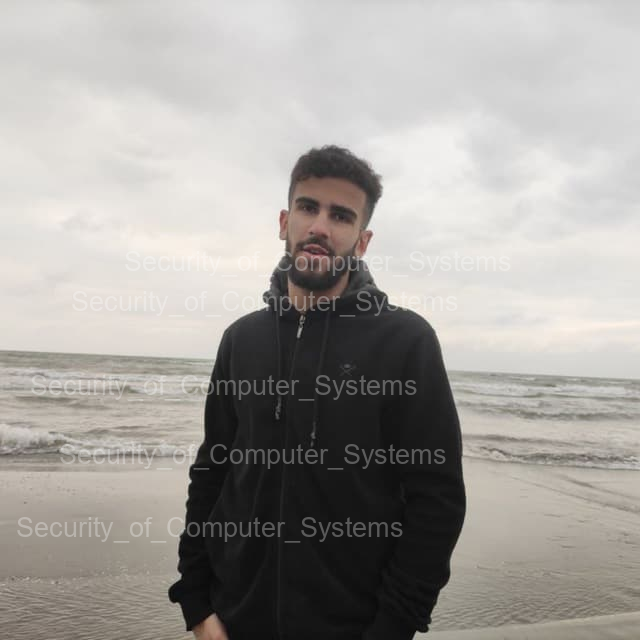
\includegraphics[width=0.7\textwidth]{Images/watermarked.png}
  \caption{تصویر \lr{watermark} شده}   
\end{figure}
سپس تصویر واترمارک شده را تحت چهار عملیات چرخش، برش، تغییر اندازه و افزودن نویز بررسی کردیم. همانطور که مشاهده می‌کنید، واترمارک‌ها از بین نرفته‌اند و نشان‌دهنده‌ی غیرشکننده و قابل مشاهده بودن آن است. 
\begin{figure}[H]
  \centering
  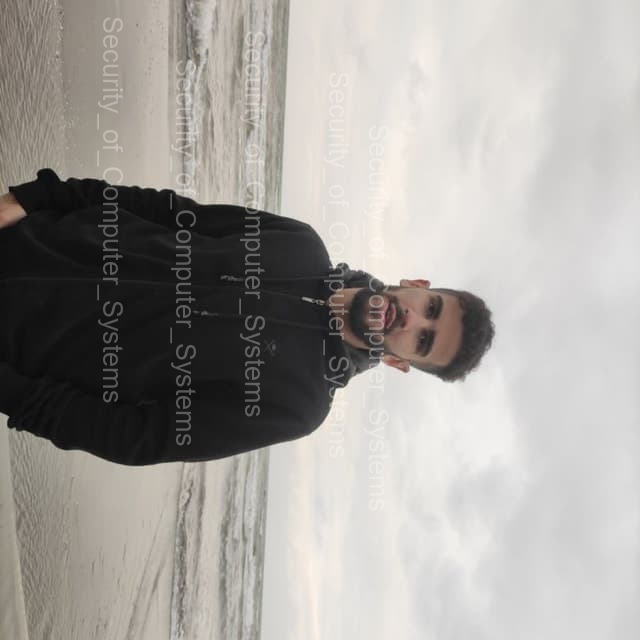
\includegraphics[width=0.7\textwidth]{Images/rotated.png}
  \caption{اعمال چرخش بر روی تصویر \lr{watermark} شده}   
\end{figure}
\begin{figure}[H]
  \centering
  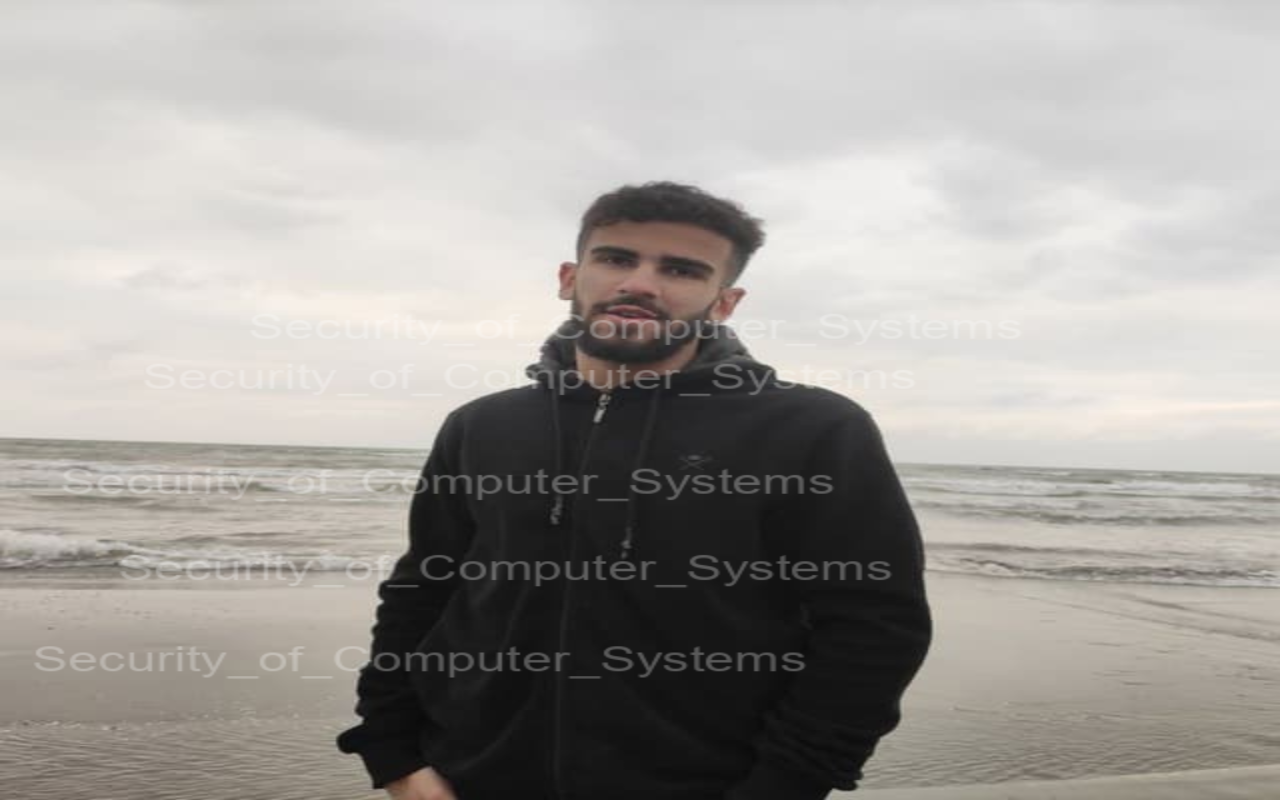
\includegraphics[width=0.7\textwidth]{Images/resized.png}
  \caption{اعمال تغییر اندازه بر روی تصویر \lr{watermark} شده}   
\end{figure}
\begin{figure}[H]
  \centering
  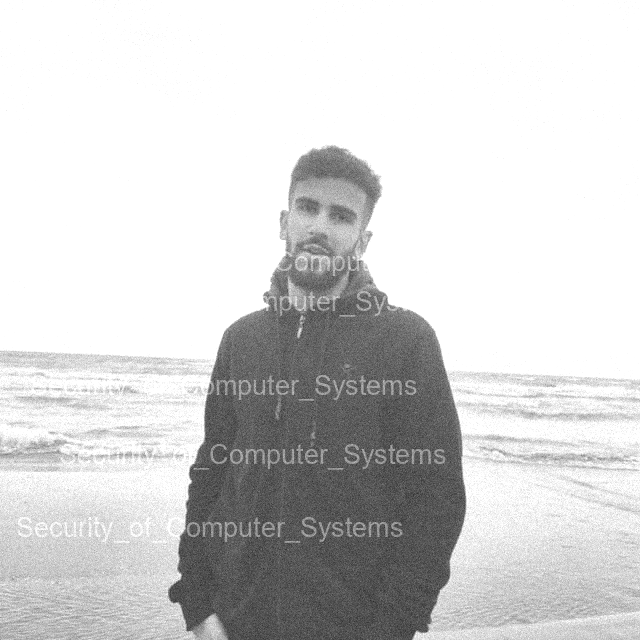
\includegraphics[width=0.7\textwidth]{Images/noisy.png}
  \caption{اعمال نویز بر روی تصویر \lr{watermark} شده}   
\end{figure}
\begin{figure}[H]
  \centering
  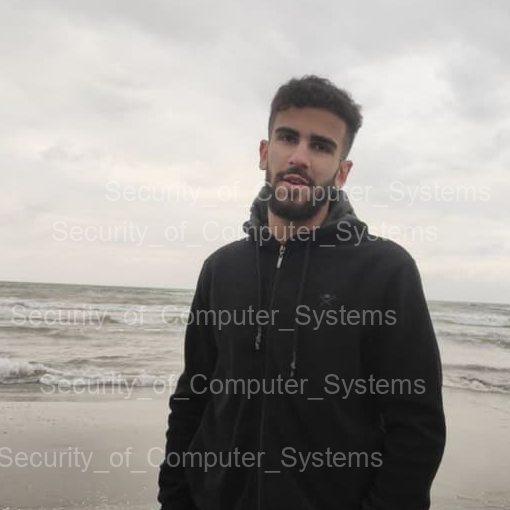
\includegraphics[width=0.7\textwidth]{Images/cropped.png}
  \caption{اعمال برش بر روی تصویر \lr{watermark} شده}   
\end{figure}
\begin{latin}
\href{https://holypython.com/how-to-watermark-images-w-python-pil/}{\textcolor{blue}{Reference}}
\end{latin}
